\documentclass[MasterThesisMain.tex]{subfiles}
\begin{document}
\appendix

\lstset{language=Matlab,%
    %basicstyle=\color{red},
    breaklines=true,%
    morekeywords={matlab2tikz},
    keywordstyle=\color{blue},%
    morekeywords=[2]{1}, keywordstyle=[2]{\color{black}},
    identifierstyle=\color{black},%
    stringstyle=\color{mylilas},
    commentstyle=\color{mygreen},%
    showstringspaces=false,%without this there will be a symbol in the places where there is a space
    numbers=left,%
    numberstyle={\tiny \color{black}},% size of the numbers
    numbersep=9pt, % this defines how far the numbers are from the text
    emph=[1]{for,end,break},emphstyle=[1]\color{red}, %some words to emphasise
    %emph=[2]{word1,word2}, emphstyle=[2]{style},    
}

\chapter{Fresnel functions and Dispersion files} \label{app:fresnel}

\section{Functions}
\lstinputlisting{fresnel_am_s.m}
\lstinputlisting{filmphasethickness.m}
\lstinputlisting{fresnel_am_tf_s.m}
\lstinputlisting{fresnel_am_tf_lay_sub.m}
\lstinputlisting{cauchy.m}


\section{10 layer model functions}
\lstinputlisting{thinfilmlayer2.m}
\lstinputlisting{thinfilmlayer3.m}
\lstinputlisting{thinfilmlayer4.m}
\lstinputlisting{thinfilmlayer5.m}
\lstinputlisting{thinfilmlayer6.m}
\lstinputlisting{thinfilmlayer7.m}
\lstinputlisting{thinfilmlayer8.m}
\lstinputlisting{thinfilmlayer9.m}
\lstinputlisting{thinfilmlayer10.m}
\lstinputlisting{thinfilmlayer11.m}
\lstinputlisting{thinfilmlayer12.m}

\section{Dispersion files curves} \label{app:dispersion}

\begin{figure}[H]
\centering
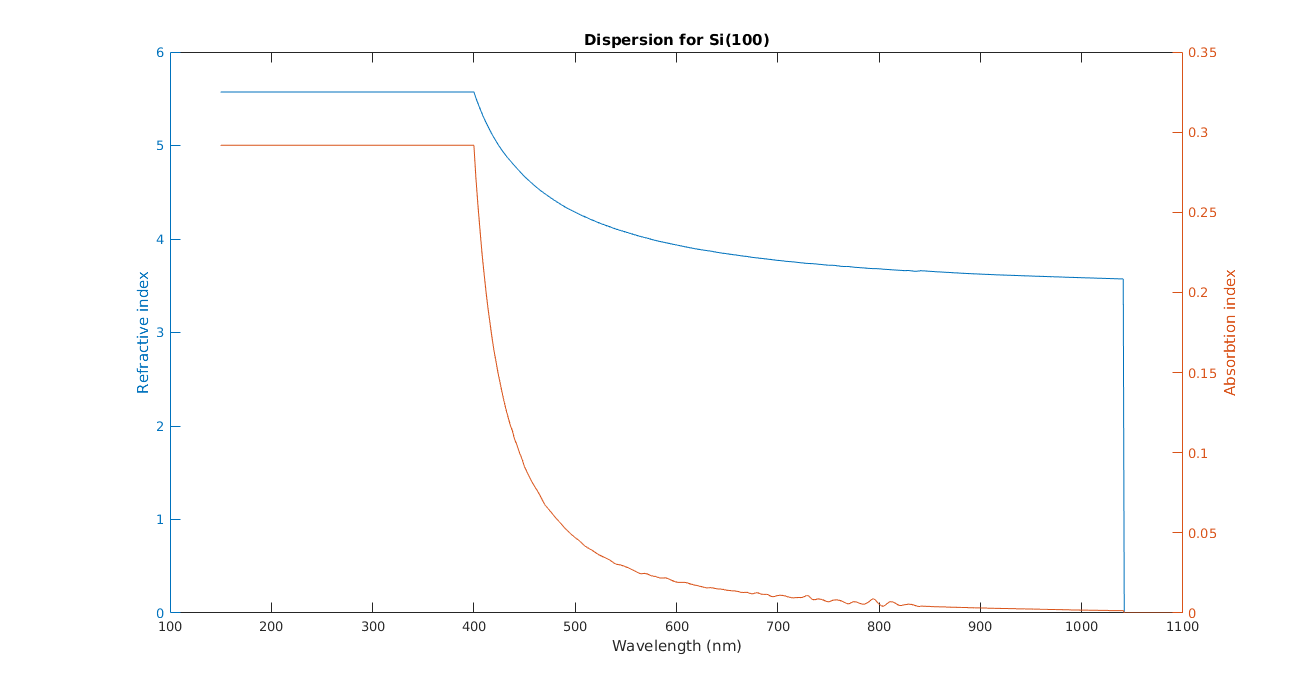
\includegraphics[width=\textwidth]{dispersionsi.png}
\end{figure}

\begin{figure}[H]
\centering
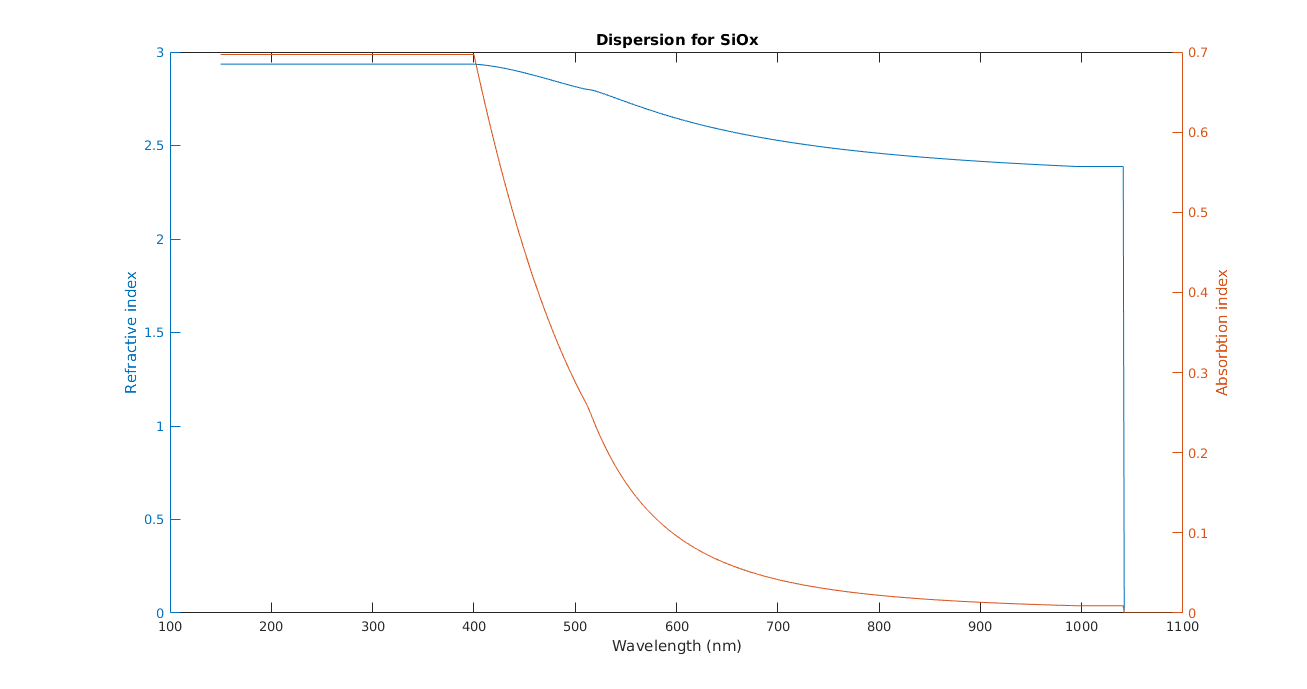
\includegraphics[width=\textwidth]{dispersionsiox.png}
\end{figure}

\lstinputlisting{dispersionfigures.m}


\chapter{Scripts}

\section{SVA Protocol - slowslow.fps}\label{app:slowslow}
\lstinputlisting{slowslow.fps}

\section{Light Source fluctuation study}\label{app:Lightstudy}
\lstinputlisting{lightplottingreflectance.m}

\section{Nano-Calc simulated reflectance curve}\label{app:simcurves}
\lstinputlisting{Script_Air_SI_Air.m}
\lstinputlisting{Script_Air_n1_5_SI_Air.m}
\lstinputlisting{Script_Air_Cauchy_SiOx_2nm_SI.m}

\section{Solvent vapour annealing ambient study}\label{app:svaambient}
\lstinputlisting{MSE_ambient.m}
\lstinputlisting{refractiveplotsambient.m}

\section{Polystyrene}
\lstinputlisting{PSMSEframevalues.m}
\lstinputlisting{PSswellingmovie.m}

\section{Polyisoprene}
\lstinputlisting{PIMSEframevalues2.m}
\lstinputlisting{PIswellingmovie2.m}

\section{Polystyrene-b-polyisoprene}
\lstinputlisting{PSPIMSEframevalues.m}
\lstinputlisting{PSbPIswellingmovie.m}






\end{document}